\subsection{经典MRC模型}
想让机器能够阅读理解文本需要解决以下几个问题:
\begin{enumerate}
	\item 如何将段落和问题这种文本形式的无结构数据表示为计算机可以处理的形式;
	\item 如何根据问题检索出段落中与问题最相关的部分;
	\item 如何从检索出来的文章片段中归纳得到答案。
\end{enumerate}
在预训练模型出现之前,
用于MRC任务的深度学习模型的整体框架主要包括如下几个层:词嵌入层、编码层、交互层、答案输出层,如图1所示。
词嵌入层的作用是将段落和问题嵌入到低维的向量空间中,用每一个向量表示每一个单词。
编码层的作用是编码段落和问题中单词的语义信息,使得每一个单词可以关注到它的上下文。交互层的作用是
将段落的语义信息与问题的语义信息融合,让模型学习到段落中与问题最相关的部分。
答案输出层的作用是从段落中查找出问题的答案。
\begin{figure}
	\centering
	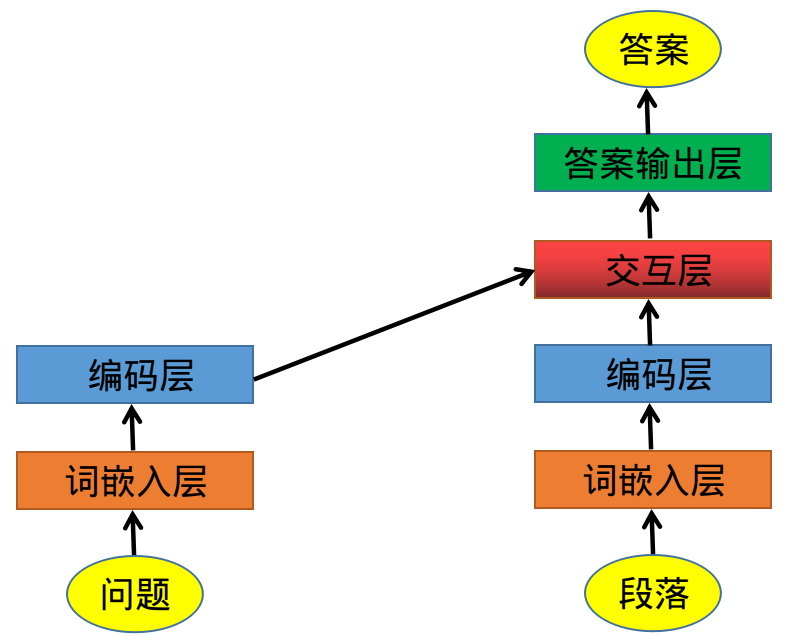
\includegraphics[width=8cm,height=7cm]{generic.png}
\end{figure}

\subsubsection{词嵌入层}
如何将文本有效的表示成计算机可以处理的形式同时可以有效地利用单词之间的语义一直的NLP领域
的重点问题。早期的one-hot形式编码用一个二值向量表示单词,但是存在数据稀疏并且随着单词个数的增加出现维度灾难的问题,此外这种形式的编码也不能够表示出单词之间的语义关系。

Rumelhart等人\upcite{Rumelhart}最早提出分布式表示的概念,
分布式表示是将单词嵌入到一个低维向量空间中用一个低维度的稠密向量表示,因此这种表示方式也叫词嵌入。语义相近的单词在向量空间中距离也相近,这种词表示方法解决了one-hot编码的很多问题。
Bengio等人\upcite{NNLM}最早将深度学习的思想融入到语言模型中提出神经网络语言模型(Neural Network Language Model,NNLM)模型,模型的第一层映射矩阵就是学习到的词向量,Mikolov等人\upcite{word2vec}受到这种思想的启发提出Word2Vec。Word2Vec提出两种模型CBOW和Skip-gram来学习单词的分布式表示,CBOW使用中心词的上下文来预测这个单词而Skip-gram利用中心词来预测其周围的单词。但是无论是CBOW还是Skip-gram都只是考虑了单词局部上下文的信息,GloVe\upcite{GloVe}利用单词共现矩阵考虑了全局统计信息。


%最流行的生成分布式词向量的技术如Word2Vec\upcite{word2vec}和GloVe\upcite{GloVe}。
大量实验表明利用Word2Vec或者GloVe预训练好的词向量作为下游任务文本的词表征来初始化下游任务模型的第一层可以显著地提升模型的效果。
除了词嵌入方法外,还有很多细粒度的嵌入方式。如Seo等人\upcite{BiDAF}提出在词嵌入的基础上结合单词的字符嵌入,以缓解NLP领域常见的OOV(out-of-vocabulary)问题。Chen等人\upcite{DrQA}提出引入单词的语义特征来增强嵌入表示,如段落单词与问题单词之间的完全匹配特征、词性特征以及单词的命名实体特征等。

然而Word2Vec和GloVe训练出来的词向量是
静态的词向量,即训练好模型后一个单词的表示
向量就是固定的,没有考虑上下文的信息,因此无法解决多义词问题。为了解决这个问题,Peters等人\upcite{ELMo}提出一种动态的基于上下文的词嵌入模型ELMo,每一个单词的词向量都是根据它所在的上下文语义表示的,很好的解决了一词多义的问题。
%ELMo\upcite{ELMo}是在2018年提出的一种动态的基于上下文的词嵌入方法。
%传统的词嵌入模型如Word2Vec\upcite{word2vec},GloVe\upcite{GloVe}属于
%静态的词向量,训练好模型后一个单词的表示
%向量就是固定的,没有考虑上下文的信息,因此无法解决多义词问题。
ELMo使用两层带有殘差连接的双向LSTM来训练语言模型,前向和反向语言模型的目标函数如公式(1)和(2)所示。
%,第一层是词嵌入层用来提取单词特征,随后是两层BiLSTM网络分别提取
%单词的词性特征和语义特征。利用语言模型作为训练任务,前向LSTM的目标是根据前$k-1$个词预测第$k$个词,如公式(10)。反向LSTM的目标是根据最后的单词直到第$k+1$个单词预测第$k$个单词,
%具体如公式(11)。
\begin{gather}
p(t_1,t_2,\cdots,t_N)=\prod_{k=1}^{N}p(t_k|t_1,t_2,\cdots,t_{k-1})\\
p(t_1,t_2,\cdots,t_N)=\prod_{k=1}^{N}p(t_k|t_{k+1},t_{k+2},\cdots,t_{N})
\end{gather}
最后的目标函数是最大化联合的前向和后向最大似然:
\begin{equation}
\begin{split}
L(\Theta)&=\sum_{k=1}^{N}(\log p(t_1,\cdots,t_{k-1};\Theta)) \\
&+\log p(t_{k+1},\cdots,t_N;\Theta)
\end{split}
\end{equation}
在做阅读理解任务时,将文章和问题输入到模型中,每一层都会得到句子的语义表示,
将每一层的特征加权求和作为下游模型的输入。
%此时得到的每一个单词的
%向量表示都是考虑了上下文的,将

%利用ELMo+BiDAF\upcite{BiDAF}
%结构超过之前单模型8.3个百分点。
%可以看出ELMo属于自回归语言模型,模型的迁移方式是基于特征的方式。
%关于ELMo以及预训练模型的细节见\ref{pretrain}节。

从早期的one-hot形式编码到分布式表示技术最后到基于上下文的词嵌入技术,每一种技术的出现都证明了一个好的文本表示方法可以
极大地提升模型的性能。
\subsubsection{编码层}
这一层的目的是在词嵌入层的基础上通过对词嵌入层的输入文本做特征提取,进一步获得句子层面的语义信息。
NLP领域最为常用的特征提取器
是基于循环神经网络(RNNs)的变体如LSTM\upcite{LSTM}和GRU\upcite{GRU}等,因为这种循环结构适合处理文本这类序列数据,绝大部分的MRC模型编码层都是利用RNNs作为特征提取器。
但是这种序列式的结构不能并行计算,训练耗时,更重要的是由于梯度消失所以不能解决单词之间长距离依赖问题,使得其
特征提取能力始终受限。Vaswani等人\upcite{Transformer}提出了一种用于机器翻译的seq2seq结构的模型transformer,舍弃了常用的循环神经网络结构,完全的基于自注意力机制构建模型,实验表明transformer的特征提取能力强于循环神经网络而且可以并行计算加快训练。
Yu等人\upcite{QANet}提出一种网络模型QANet,不像之前的那些模型几乎都是用RNNs来做编码器,
QANet提出一种新颖的编码结构,利用卷积结合transformer\upcite{Transformer}中的
多头注意力结构
。
%卷积方式采用的是文献\cite{DSC}提出的深度可分离卷积(depthwise 
%separable convolutions),
%相比传统的卷积计算方式深度可分离卷积可以减少运算次数。
整个结构的思想是先利用卷积建模局部特征的交互,再用自注意力机制建模全局交互,
实验结果表明这种架构不仅加快训练速度同时在SQuAD数据集上模型性能优于那些利用RNNs作为编码器的模型。
关于transformer的细节介绍见\ref{transformer}节。


%每一层由多头自注意力和前馈网络(FN)构成。Transformer的整体架构
%通过利用自注意力(self-attention)机制取代RNN那种序列式的计算方式,
%对于一个句子中的两个单词不考虑单词之间顺序的关系,直接计算它们之间的相关度,例如计算两个单词向量表示的内积。
%自注意力机制可以捕获句子中长距离依赖的特征关系,
%解决了循环神经网络固有的序列式传递信息导致后面的单词与前面的单词
%之间达不到有效的信息传递问题。
%通过自注意力机制不仅可以做到
%单词之间的全局交互同时其并行计算使得模型训练时间大幅减少。Transformer的encoder端和decoder端都可以做特征提取器如BERT\upcite{BERT}用encoder端特征提取,GPT\upcite{GPT}用decoder端特征提取,实验证明在大规模数据集上transformer的特征提取能力要强于
%基于RNNs\footnote{用RNNs来统一表示RNN的变体,如LSTM,GRU等\label{RNNs}}的编码器,目前几乎所有的NLP预训练模型都是利用transformer作为特征提取器。

\subsubsection{交互层}
%在预测答案时需要将问题的语义信息与文章的语义信息关联,这样模型在预测答案时才能知道文章中哪一部分是问题的答案。
%通常利用注意力机制实现这一目的,注意力机制就是让模型关注到重点的部分,不同的注意力计算方式很大程度上影响模型性能,
%后面将详细介绍基于注意力机制的模型以及它们不同的计算方式。
交互层是整个网络模型中关键的一层,
%前面的编码层输出的是问题和段落中每个单词的上下文语义表示,每个单词
%关注了自己所在句子的上下文单词,但是却并没有关注对应的句子。而人们在做阅读理解问题时,通常是带着
%问题去文章中找答案,我们要知道文章中每一个单词和问题之间的相关度。因此交互层的
目的就是让段落的语义信息与问题的
语义信息融合,达到对段落更深层次的理解,而交互层中最常用的方法就是注意力机制(Attention)。

注意力机制可以被视为是一个查询向量(query)和一组键值对向量(key-value pairs)的映射过程。整个过程首先是利用函数$f$衡量query和key之间的相似度,生成一个权重分数向量,然后将权重分数向量归一化(通常利用softmax函数)后对value加权求和,得到的结果就是query对key-value pairs的注意力。具体计算公式形式如下:

\begin{gather}
\alpha_i=\text{softmax}(f(Q,K_i)) \notag \\
\text{Attention}(Q,K,V)=\sum_{i=1}^{n}\alpha_iV_i
\end{gather}
其中$Q$表示query的向量表示,$(K_i,V_i)$代表key-value pairs向量表示的第$i$个值,
函数$f$常采用计算方式有内积、二次型函数、
前馈神经网络,双维度转换函数,分别见如下公式:
\begin{gather}
f(p_i,Q)=p_i^TQ \qquad \text{内积} \\
f(p_i,Q)=p_i^TWQ\qquad \text{二次型函数}\\
f(p_i,Q)=v^T\tanh(Wp_i+UQ)\qquad \text{前馈神经网络} \\
f(p_i,Q)=p_i^TW^TUQ \qquad \text{双维度转换函数}
\end{gather}

在NLP领域中$K=V$,即对于两个序列,其中一个序列为另一个序列的每一个位置生成一个权重值,这个值代表当前位置的单词对另一个序列的重要性。
如果是自注意力(self attention),那么$Q=K=V$,目的是计算序列中某个单词和其它单词之间的相关性从而增强自身的语义表示。
Bahdanau等人\upcite{Bahdanau}最早将
注意力机制应用在机器翻译领域,获得了极大的反响,
为NLP领域的其它任务的模型提供了启发式的思想。

MRC模型做注意力运算有两个方向:从问题到段落(Question-to-Context,Q2C),从段落到问题(Context-to-Question,C2Q)。Q2C的注意力是指
将问题看做是$Q$,段落看做$K,V$。定义$C=[c_1,c_2,\cdots,c_n] \in R^{n\times d}$代表段落的表示向量,其中$n$代表段落单词的个数,$d$代表向量维度,
$Q\in R^{d}$代表整个问题的表示向量
%利用问题去和段落做注意力计算,
%得到问题对文章的注意力权值,它代表问题对文章每一个单词的关注程度,利用它对段落的表示向量加权求和得到的就是问题的一个新的表示向量。
%以Q2C的注意力计算过程为例,
%每一个
%$p_i$代表文章中单词的语义向量表示,$Q$代表整个问题的语义信息。
Q2C的注意力计算步骤如下:
\begin{gather}
\alpha_i=\text{softmax}(f(c_i,Q)) \notag \\
\text{Attention}(C,Q)=\sum_{i=1}^{n}\alpha_{i}c_i
\end{gather}
%就是利用问题
%的语义信息和文章中每一个单词的向量表示计算它们之间的相关性,最后得到一组注意力权重$\alpha=[\alpha_1,\alpha_2,\cdots,\alpha_n]$
%表示文章与问题之间的相关程度,利用$\alpha$对文章加权求和就可以提取出来文章中与问题最相关的单词,
%这些单词对于回答问题是至关重要的。
计算得到的$\text{Attention}(C,Q)$也叫段落感知的问题表示(context-aware query representation)。
C2Q注意力的计算方式类似,段落看作是$Q$,问题看做$K,V$,计算得到的$\text{Attention}(C,Q)$也叫问题感知的段落表示(query-aware context representation)。
%拿段落和问题做注意力计算,段落的每一个单词都会
%关注到问题,然后利用注意力权值对问题加权求和从而计算得到段落的新的表示向量。

公式(9)是将问题压缩成一个固定维度的向量,得到的注意力权重$\alpha$也是一维的,因此也称为一维注意力。
一维注意力方法所关注的是问题序列的整体对文章的注意力,没有考虑问题序列的不同单词之间对文章的关注程度差异。
与其相对应的是二维注意力,即对于问题序列中的
每一个单词都会和段落做注意力计算,得到的注意力权重是二维的。

%段落到问题注意力可以看做是带着文章阅读问题,问题到段落则可以看做是带着问题阅读文章。
%C2Q和Q2C这两种都属于交互的计算注意力,然而这种注意力机制可能导致只重视文章中与问题相关度高的单词,而忽视了文章所强调自身的语义信息。在文章上利用自注意力机制则可以看做是反复的阅读文章,从而加深对文章语义信息的理解。



此外还可以将注意力机制分为one-hop和multi-hop形式。其中one-hop也叫“单跳结构”,是指仅仅通过一次计算得到注意力权值然后加权求和得到注意力结果
%,这也是一种静态的计算形式
。与之对应的是multi-hop,也叫“多跳结构”,one-hop形式下仅仅只做一次交互计算
%,而注意力机制虽然可以提取相关的重要信息,但是
%它仍然是基于浅层语义信息的相似度计算。在机器阅读理解任务中,
,而对于复杂的问题通常是不能在一个句子中找出答案,需要在多个句子甚至多篇文章中多次推理,每一步推理过程中都会变换注意力关注的对象。
%,如表6所示
%\begin{figure}[ht]
%	\centering
%	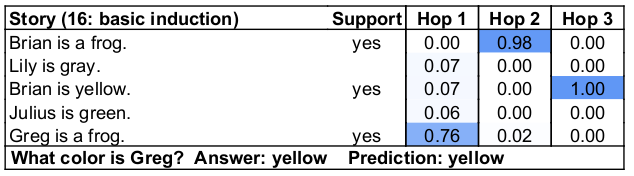
\includegraphics[width=0.5\textwidth]{end2end.png}
%	\caption{MemN2N\upcite{MemN2N}提出的多步推理的一个样例 \\ Figure 1 An example of multi-hop reasoning from MemN2N}
%\end{figure}

%\begin{table}[ht]
%	\centering
%	\caption{MemN2N\upcite{MemN2N}提出的多跳推理样例}
%	\begin{tabular}{l}
%		\toprule
%		Brian is a frag. \\
%		Lily is gray. \\
%		Brian is yellow. \\
%		
%	\end{tabular}
%\end{table}

%\begin{table}[ht]
%	\centering
%	\caption{WIKIHOP\upcite{WIKIHOP}多跳推理的样例}
%    \begin{tabular}{l p{15.0cm}<{\raggedright}}
%	\toprule
%	文章1:&\tabincell{l}{The Hanging Gardens, in \textcolor{blue}{[Mumbai]}, also known as Pherozeshah
%		Mehta Gardens, are terraced gardens …  \\
%		They provide sunset views
%		over the \textcolor{red}{[Arabian Sea]} …} \\
%
%	文章2:&\tabincell{l}{\textcolor{blue}{Mumbai} (also known as Bombay, the official name until 1995) is the
%		capital city of the Indian state of Maharashtra. \\It is the most
%		populous city in \textcolor{green}{India} …}\\
%	%\cmidrule(l){2-3}
%	文章10:&\tabincell{l}{The \textcolor{red}{Arabian Sea} is a region of the northern Indian Ocean bounded
%		on the north by \textcolor{magenta}{Pakistan} and \textcolor{magenta}{Iran}, \\ on the west by northeastern
%		\textcolor{magenta}{Somalia} and the Arabian Peninsula, and on the east by India …}\\
%	\hline
%	问题:&Hanging gardens of Mumbai, country,? \\
%	%\cmidrule(l){2-3}
%	\midrule
%	答案:&{Iran, \textcolor{green}{India}, Pakistan, Somalia} \\
%	\bottomrule
%\end{tabular}
%\end{table}                     
% \begin{figure*}
%     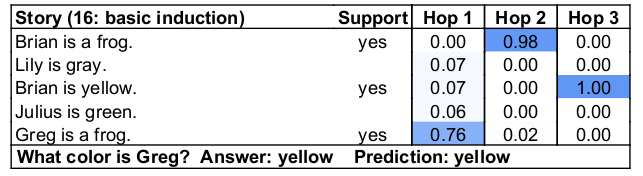
\includegraphics[]{multihop.png}
% \end{figure*}
%当前时刻计算的注意力结果要保留到下一时刻,即每一时刻都要计算注意力,是一种动态的计算形式,典型的代表是Bahdanau注意力\cite{neural machine translation by jointly learning to align and translate}。
%我们可以看到想要得到最终的答案需要在多个段落中进行多次推理,
%在每一个推理过程中都会变换注意力关注的对象,显然one-hop结构是不能实现多步推理的。

鉴于目前多数模型交互层所使用的注意力机制较为复杂,很难按照上述形式完全的区分开每一个模型,本文按照Liu等人\upcite{Survey}的思路按照注意力计算的方向等划分各个模型。
\vspace{1ex}

\noindent\textbf{单向注意力} \quad Hermann等人\upcite{Hermann}最早利用神经网络模型并且融入注意力机制做MRC任务。
文中提出两种不同的单向注意力机制模型Attentive Reader
和Impatient Reader,均是计算问题到文章(Q2C)的注意力,且注意力的运算方式采用前馈神经网络(公式4)。
%不同之处在于Attentive Reader属于一维注意力,Impatient
%是将问题表示为一个固定长度的向量然后与文章中每一个单词做注意力计算,然后利用注意力权重对文章
%中的单词的向量表示加权求和得到一个固定长度的
%向量即为注意力运算后的结果,然后与问题联合预测答案,其中注意力的运算方式采用前馈神经网络(公式4)。
%可见这种注意力的计算方式仅仅只计算一次,因此属于one-hop类型。
Chen等人\upcite{AR}在Attentive Reader的基础上利用双线性项(公式3)取代原有的前馈神经网络计算方式。
%并且直接将对段落加权求和后得到的向量作为预测答案的输入而不是联合问题$Q$的语义信息,实验证明这种简化反而提高了模型的准确度。
类似的,Kadlec等人\upcite{ASR}利用内积运算作为注意力计算方式。
%Wang等人\upcite{MatchLSTM}提出Match-LSTM模型,
%与之前的模型不同,Match-LSTM计算的方向是段落到问题(C2Q)的注意力,目的是将问题的语义信息融入到Match-LSTM网络中。其它相关的基于单向注意力机制的模型可以参考IA Reader\upcite{IAReader},AS Reader\upcite{ASR}等。
%具体计算过程如下:
%\begin{gather}
%s_t=v^T\tanh(W^QH^Q+W^Ph_t^P+W_rh_{t-1}^r) \notag \\
%\alpha_{t}=\text{softmax}(s_t)
%%c_t=\sum_{i=1}^{m}a_i^tu_i^Q
%\end{gather}
%其中$H^Q$是问题通过编码层的输出,$h_t^P$是段落的第$t$个单词通过编码层的输出,$h_{t-1}^r$是Match-LSTM上一时刻
%的隐藏状态。
%$\alpha_{t}$是
%段落的第$t$个单词与问题的每一个单词之间的注意力权重。
%计算得到的注意力权重对问题的语义表示加权求和,然后与段落当前时刻单词的上下文表示拼接作为
%Match-LSTM当前时刻的输入。
%\begin{gather}
%z_t=[h_t^p;\alpha_tH^q] \notag \\
%h_{t}^r=\text{LSTM}(z_t,h_{t-1}^r)
%\end{gather}
%此外为了使得段落从后向前的对问题做关注,模型将段落序列翻转再次按照上述方式计算,最后将两个方向的计算结果
%拼接作为交互层的输出。
\vspace{1ex}

%上述的模型要么仅计算C2Q方向的注意力或者仅计算Q2C方向的注意力
\noindent \textbf{双向注意力} \quad 单向注意力所能交互的信息有限,而双向注意力则可以达到两个方向的互补,提供更加全面的交互信息。
Xiong等人\upcite{DCN}提出Dynamic Co-attention Network(DCN)模型,
在交互层中采用协同注意力机制,
协同注意力同步的计算C2Q以及Q2C两个方向的注意力,
最后融合两个方向的注意力作为交互层的输出。
%\begin{equation}
%\widetilde{C}=\beta[Q,\alpha C]
%\end{equation}
%其中$\alpha$和$\beta$分别表示段落与问题之间的注意力权重,$\widetilde{C}$同时融合了问题的语义信息和段落的语义信息。
Seo等人\upcite{BiDAF}提出(Bidirectionl Attention Flow,BiDAF)模型。
同样计算两个方向(C2Q和Q2C)的注意力,但是与之前模型不同的是BiDAF将之前的段落语义表示和交互层计算得到的问题感知的段落语义表示一起流向后面的层,这样一定程度上避免了过早的对段落语义信息概括而导致
信息的损失。模型的简化实验表明C2Q方向的注意力对模型的重要性大于Q2C方向的注意力,一种可能的原因是由于问题序列的长度小于段落文本的长度所以计算得到的段落感知的问题语义向量的信息不够充分。
\vspace{1ex}

\noindent \textbf{单跳结构} \quad 单跳
结构是指段落与问题之间的交互仅仅计算一次。
%得到注意力权值然后加权求和得到注意力结果,
要么是将问题整体压缩为一个向量与段落计算一次注意力,如Attentive Reader\upcite{Hermann},AS Reader\upcite{ASR}等,或者问题与段落的的整体表示采用并行化的计算方式,如DCN\upcite{DCN},BiDAF\upcite{BiDAF}等。
\vspace{1ex}

\noindent \textbf{多跳结构} \quad 单跳结构不能实现多步推理的效果,多跳结构可以视为单跳结构的堆叠,目的是通过多次计算段落与问题的交互信息加深模型对段落和问题的理解,从而达到多步推理的目的。
实现多步推理这种机制通常有以下几种方式:
\vspace{1ex}

\noindent 第一种方式是基于之前时间步所计算得到的问题感知的段落表示,计算下一时间步的段落和问题交互,以一种序列式的方式计算注意力,如Impatient Reader\upcite{Hermann},
%并不是像Attentive Reader将
%	问题表示为一个固定长度的向量,而是对于问题中的每一个单词都要和整个段落做注意力计算,而且计算的结果
%	要和下一个单词以及段落共同做注意力计算,最后一个单词的注意力结果作为整个Impatient Reader计算注意力过程的输出。
这种方式类似于人在阅读过程中不断的在问题和文章之间做关注。
\vspace{1ex}

\noindent
第二种方式是利用RNNs这种基于上一时刻隐藏状态更新下一时刻隐藏状态的循环特性来达到多步推理,
如Wang等人\upcite{MatchLSTM}提出的Match-LSTM模型,序列式的阅读段落,利用LSTM存储每个时间步计算得到的问题感知的段落表示。具体的,计算段落当前时刻的单词与问题的注意力,得到的问题感知的段落表示与当前时刻段落单词的向量表示拼接作为LSTM的输入。
类似的模型如RNet\upcite{RNet},IA Reader\upcite{IAReader}等
%利用BiGRU存储每一次迭代计算得到的问题和段落的交互信息。
%在每一时间步上,首先利用上一次的BiGRU的状态与问题做一维注意力匹配提取出问题的语义信息,
%然后再结合上一次的BiGRU的状态与段落再做一维注意力匹配从而提取出段落的语义信息。将问题与段落的语义信息
%通过各自的门控单元作为BiGRU当前时刻的输入,其中门控单元采用前馈神经网络用来解决当前时间步下问题和段落的语义信息提取不充分的问题。
%基于注意力机制的模型大部分是利用RNN的循环机制来存储每次交互的状态,
%但是由于RNN的梯度消失问题可能会丢失语义信息,因此文献\cite{memory network}提出一种记忆网络架构(memory network),
%通过外部记忆模块来存储语义信息,但是这种记忆网络并不能端到端的训练。
%为了处理这个问题,文献\cite{MemN2N}提出一种端到端的记忆网络(MemN2N)。
%利用记忆槽存储文档中每一个句子的嵌入矩阵,记忆槽的状态以及问题的语义信息会随着与文档的多次交互不断更新。
\vspace{1ex}
%

\noindent
第三种方式通过堆叠多个计算注意力的层数达到多步推理的目的,
如Dhingra等人\upcite{GAReader}提出的Gated Attention Reader(GA Reader)模型,类似于IA Reader模型,同样采用
BiGRU作为编码模块实现多跳结构。在每一步的推理过程中,首先通过BiGRU得到问题的向量表示,然后与段落的
每一个单词做注意力的计算得到问题感知的段落表示
%同时采用点乘计算的门控机制建模问题感知的段落表示和原来的段落语义向量之间的交互关系,目的是利用问题更新文章的语义表示。
作为下一层BiGRU的输入,
这种处理过程类比于带着问题反复的阅读文章,每一次都加深对文章的语义理解。
%Wang等人\cite{RNet}提出一种带有门控机制的注意力循环神经网络以及自注意力机制联合的交互层设计模型RNet。RNet在交互层的设计分为两部分。
%第一部分是带有门控机制的注意力循环神经网络,整体计算
%方式类似于Match-LSTM,而且额外加入了门控机制使得模型可以有选择的输出
%语义信息。具体的,在公式(7)中的$z_t$上添加一个门控单元:
%\begin{gather}
%g_t=\text{sigmoid}(W_gz_t)\notag \\
%z_t^{*}=g_t\odot z_t
%\end{gather}
%其中$\odot$表示元素之间的点乘。
%%由于$z_t=[h_t^p;\alpha_tH^q]$,$h_t^p$表示的是文章的第$t$个单词的语义表示,$\alpha_tH^q$表示的是
%%对问题语义表示的融合,因此
%通过添加门控单元使得模型可以有选择的决定哪部分作为重要的语义信息输出。这种机制类似于人在阅读过程中要
%忽略段落中那些与问题无关的信息,凸显出重要的信息才能更加准确的找到答案。
%第二部分是利用自注意机制对段落的语义信息再次交互建模,
%%基于注意力机制的循环神经网络的输出对关注了问题的
%%文章语义表示与原始文章语义表示建模后的输出,而这种计算机制的问题之一是
%%两个距离较远的单词之间交互信息由于梯度消失等原因会变得很弱。因此
%通过自注意机制可以使得段落中每一个单词关注到其余所有的单词,使得模型对段落达到更深层次的理解。

\noindent 之前的模型在交互层利用注意力机制融合段落和问题时都是利用句子的高层级别的语义信息而忽略了句子在低层次级别的语义信息,如单词级别的词嵌入等。
Huang等人\upcite{Fusionnet}提出FusionNet模型,将每一个单词在第一层到后面所有层的向量表示拼接成一个向量,原文中称为单词历史(history of word),因为它包含了一个单词所有层的语义编码。
%但是随着层数的增加维度会变得越来越大,
为了解决维度问题同时不损失单词的历史信息,FusionNet提出全关注注意力机制的概念:利用段落和问题的单词历史计算得到注意力权重,然后对问题的某一层表示向量加权求和。这种机制使得两个输入向量可以互相关注到对方的历史信息同时压缩维度,文中对注意力权重的计算方式如下:
\begin{equation}
\alpha_i=\text{ReLU}(Up_i)^TD\text{ReLU}(Uq_j)
\end{equation}
其中$p_i\in R^d$和$q_j\in R^d$分别代表段落第$i$个单词和问题第$j$个单词的单词历史,$U$和$D$是训练的参数。
%第三种方式是引入额外的记忆单元存储语义信息,目的是希望解决RNN中不能够长期依赖导致信息丢失的问题,典型
%	的如Weston等\upcite{MN}
%	提出的记忆网络(memory networks)。
%

\noindent Hu等人\upcite{RMR}认为在多层架构中,当前层的注意力计算并没有直接考虑到之前层计算得到的注意力信息,这可能导致两个不同但是相关的问题:(1)多层注意力分布集中在相同的文本上导致注意力冗余;(2)多层注意力未能集中在文本的重要部分造成注意力缺乏。针对这两个问题他们提出强化助记阅读器(Reinforced Mnemonic Reader,RMR)模型,利用重关注机制,通过直接利用之前层计算的注意力信息来微调当前层注意力分布的计算。

除了上面介绍的一些模型外,还有一些基于上述模型中注意力机制改进的模型,如Wang等人\upcite{RNet}提出的RNet模型,在Match-LSTM的基础上添加门控机制,将问题感知的段落表示与段落单词的向量表示拼接后通过一个门控单元。
通过添加门控机制使得模型决定哪部分作为重要的语义信息输出。这种机制类似于人在阅读过程中要
忽略段落中那些与问题无关的信息,凸显出重要的信息才能更加准确的找到答案。
此外RNet利用自注意机制对段落表示进行自注意力计算,
尽管利用基于注意力机制的循环神经网络可以存储中间过程计算得到的问题感知的段落表示,
%的输出对关注了问题的
%%文章语义表示与原始文章语义表示建模后的输出,而这种计算机制的问题之一是
但是两个距离较远的单词之间的交互信息由于梯度消失等原因会变得很弱。因此
通过自注意机制可以使得段落中每一个单词关注到其余所有的单词,使得模型对段落达到更深层次的理解。

Shen等人\upcite{Reasonet}提出一种动态决定推理次数的模型ReasoNet,不同于IA Reader,GA Reader等模型,在整个推理过程中有着固定的推理次数。这种固定推理次数的缺点就是不考虑问题的复杂性。
%对于复杂的问题往往需要模型多次的推理,因此不同题目难度需要不同的推理次数,应当让模型学会什么时候终止推理。为了达到这一目的,
ReasoNet模型利用一个终止门产生二元值输出来动态的决定是否继续推理。ReasoNet模型大致分为外部记忆单元模块、内部控制器模块、终止门模块以及答案输出模块。
将段落和问题通过Bi-GRU编码后的语义表示作为
外部的记忆单元$M$,利用内部控制器(采用GRU)当前时刻的状态与$M$做二维注意力匹配,得到注意力结果输入到内部控制器中
更新内部控制器的状态。终止门模块以当前时刻内部控制器的状态作为输入来判断是否需要继续推理。由于产生了二元离散输出值,
使得模型不能用梯度下降法训练,因此模型引入强化学习机制训练。

表7对比了本节介绍的经典的MRC模型在注意力机制设计上的差异。其中Q2C代表问题到段落注意力,C2Q代表段落到问题注意力,Bidirectional代表双向注意力,self-attention代表对段落做自注意力运算,one-dim代表一维注意力,two-dim代表二维注意力,one-hop代表单跳结构,multi-hop代表多跳结构。
\begin{table}[ht]
	%\text{基于注意力机制的模型对比}
	\centering
	\caption{基于注意力机制的模型对比 \\ Table 7 Comparison of models based on attention mechanism}
	%\vspace{10pt}
	%\resizebox{\linewidth}{!}{
	\begin{tabular}{c c c c}
		\toprule
		模型&注意力方向&注意力维度&推理模式 \\
		\midrule
		Attentive Reader\upcite{Hermann}&Q2C&one-dim&one-hop \\
		\midrule
		Impatient Reader\upcite{Hermann}&Q2C&two-dim&multi-hop \\
		\midrule
		Standford Reader\upcite{AR}&Q2C&one-dim&one-hop \\
		\midrule
		AS Reader\upcite{ASR}&Q2C&one-dim&one-hop \\
		\midrule
		IA Reader\upcite{IAReader}&Q2C&one-dim&multi-hop \\
		\midrule
		GA Reader\upcite{GAReader}&C2Q&two-dim&multi-hop \\
		\midrule
		Match-LSTM\upcite{MatchLSTM}&C2Q&two-dim&multi-hop \\
		\midrule
		DCN\upcite{DCN}&Bidirectional&two-dim&one-hop \\           
		\midrule
		BiDAF\upcite{BiDAF}&Bidirectional&two-dim&one-hop \\
		\midrule
		ReasoNet\upcite{Reasonet}&Bidirectional&two-dim&multi-hop\\
		\midrule
		R-Net\upcite{RNet}&C2Q+self-attention&two-dim&multi-hop \\
		\midrule
		RMR\upcite{RMR}&Q2C+self-attention&two-dim&multi-hop \\
		\midrule
		QANet\upcite{QANet}&Bidirectional&two-dim&one-hop\\
		\bottomrule
	\end{tabular}
	%}
\end{table}



\subsubsection{答案预测层}
这是整个模型架构的最后一层,用来输出预测的答案。MRC任务按照答案形式的不同大致分成四类,因此这一层的设计需要
考虑到答案形式。
%对于填空型任务,答案的输出是文章中的一个单词。对于多项选择任务,答案的输出是从多个候选答案中选择出正确的选项。
%对于片段选择型任务,答案的输出是文章中某段连续的文本。对于自由答案型任务,答案的输出不限固定的文本,而是根据词典中的单词生成文本。
%此外还有不可回答的问题,此时模型的输出还要考虑到问题是否可以回答。
%%答案预测层的设计细节见\ref{output}节。
%
%答案预测层的设计要依据答案的形式而设计,
下面介绍
各个模型在四类不同的MRC任务上输出层的设计。


1)填空式:这类任务答案的形式是预测问题中缺失的单词,而且缺失的答案来源于文章中。Hermann等人\upcite{Hermann}
最早提出将问题的表示与问题感知的段落表示拼接成一个向量然后映射到整个词典中预测那个缺失的单词。
这种方法存在的一个问题就是不能够确保预测的单词一定是段落中的词汇,
这就使得模型的预测准确率受到影响。指针网络(Pointer networks\upcite{Ptr})模型由seq2seq模型演变而来,主要就是
为了解决输出源自于输入的问题,实现方式是利用计算的注意力权重分布直接输出预测结果,而这种机制正适合
填空式任务以及抽取式任务。
Kadlec等人\upcite{ASR}提出AS Reader模型正是受到指针网络的启发,对于计算得到的注意力权重分布,将其中相同单词的注意力
权值相加,最后输出具有最大权值的单词最为答案。
填空式任务下,模型的损失函数可以写
为$L(\theta)=-\displaystyle\frac{1}{N}\sum_{i=1}^{N}\log P_{y_i}$。
其中$\theta$为模型参数,$N$代表样本数目,$y_i$表示第$i$个样本中标准答案的位置。

2)多项选择式:这类任务是从多个候选答案选项中选择正确的选项。处理这种任务最简单的一种方式就是计算模型输出后的
段落表示和选项之间的相似程度,相似程度最高的作为预测的选项,从而将多项选择式任务变为句子之间的语义匹配问题。
Wang等人\upcite{Co-matching}提出将问题、段落、选项一起放在模型中做交互计算,交互层输出一个向量作为输出层的输入,
输出层采用简单的输出维度是1的全连接层,输出的值代表模型对这个选项的打分值,其它的选项类似的处理,值最高的选项作为预测的答案。
%最后对所有选项的打分值
%做归一化作为模型的训练目标。
多项选择式任务下,模型的损失函数可以写为
$L(\theta)=-\displaystyle\frac{1}{N}\sum_{i=1}^{N}\sum_{j=1}^{m}\log P_{y_{j}^i}$。
其中$\theta$为模型参数,$N$代表样本数目,$m$代表选项个数,$y_{j}^i$表示第$i$个样本中第$j$个选项是正确答案。

3)抽取式:这类任务是从文章中提取出来一段连续的单词作为答案,虽然类似于填空式任务输出来源自输入的性质,但是
不像填空式任务仅仅只是预测一个单词。因此填空式
任务答案输出层的设计不能直接用来作为抽取式任务的答案预测层。
由于提取文本的长度不固定,使得这一任务更具有挑战性。
Wang等人\upcite{MatchLSTM}同样受到指针网络的启发提出了两种基于指针网络的输出模型,第一种是序列式模型,利用指针网络以一种序列式的形式预测答案的每一个位置,处理过程类似于seq2seq模型的解码过程。
%这种模型下答案的每一个单词可能出现在文本段落的任何一个位置,
%这是因为指针网络并没有要求从输入中选择的输出具有连续性。由于答案的长度不固定,因此在段落中设置一个特殊的
%位置表示答案的终止点,当预测到这个位置时终止答案的生成。
第二种是边界式模型,不同于序列式模型那样序列的生成答案的每一个位置,由于要预测的答案是一段连续的文本,
因此可以利用指针网络仅仅预测答案的起始位置和终止位置。所预测答案的概率
是预测这两个位置概率的乘积,这种方式相比于
第一种更加的简单而且实验结果表明更加高效。


边界式模型的这种设计思想也被后来很多MRC模型采纳。尽管边界式模型简单有效,
%但是在文章中可能有些文本片段与标准答案相似,比如初始位置一样,
但是边界式模型有可能陷入局部极值的情况从而提取错误的文本片段。为了处理这个问题,Xiong等人\upcite{DCN}
提出一种动态迭代的指针网络作为解码端,利用上一次预测的答案的起始位置和终止位置以及解码端当前的状态来重新评估
下一次预测答案的起始位置和终止位置。多次迭代后选取所有迭代次数中概率最大的情形作为预测答案。
抽取式模型的损失函数可以写为
$L(\theta)=-\displaystyle\frac{1}{N}\sum_{i=1}^{N}\log P_{y_i^s}^S+\log P_{y_i^e}^E$。
其中$\theta$为模型参数,$N$代表样本数目,$y_i^s$表示第$i$个样本中标准答案的起始位置在文章中的位置,
$y_i^e$表示第$i$个样本中标准答案的终止位置在文章中的位置。
%如果考虑到不可回答的问题,最简单的方式是额外在输出层加上一个输出维度是1的全连接层。
%此时的损失函数可以写为
%$L(\theta)=-\displaystyle\frac{1}{N}\sum_{i=1}^{N}(\log P_{y_i^s}^S+\log P_{y_i^e}^E)+\log P_{y_i^u}^U$。
%其中$y_i^u$表示第$i$个样本中的问题是不可回答的问题。关于带有不可回答问题的阅读理解任务细节见\ref{unknown}节。

4)自由答案式:这类任务的答案形式已经不再是原文中某段文本,而是需要根据文章和问题生成符合语法规范的文本。
这类任务对答案生成模块的能力要求较高。处理生成任务典型的架构是seq2seq模型,将段落看做是encoder端的输入,decoder端根据词汇表中的单词生成答案。还有一类经典的处理生成任务的架构是See等人\upcite{PGNet}提出
的指针生成网络模型(Pointer-Generator Network,PGNet),最早用在文本摘要领域,模型结合了seq2seq的
生成机制以及指针网络的拷贝机制,使得模型既能从词典中生成单词又能在原文中拷贝单词,实验结果表明该模型的效果优于传统的seq2seq模型。

表8对比了经典的MRC模型在SQuAD\upcite{SQuAD1}数据集上的表现\footnote{统计数据源自Yu等人\upcite{QANet}}。


\begin{table}[ht]
	\centering
	\caption{模型在SQuAD\upcite{SQuAD1}数据集上的对比(acc代表准确率)}
	%\vspace{10pt}
	\begin{tabular}{l c}
		\toprule
		模型&EM/F1\\
		%\cmidrule(lr){2-2} \cmidrule(lr){3-3} \cmidrule(lr){4-4}
		%&EM/F1&EM/F1& acc \\
		\midrule
		Match-LSTM\upcite{MatchLSTM}& 64.7/73.7\\
		\midrule
		DCN\upcite{DCN}& 66.2/75.9\\
		\midrule
		BiDAF\upcite{BiDAF}&68.0/77.3\\
		\midrule
		ReasoNet\upcite{Reasonet}&70.6/79.4\\
		\midrule
		R-Net\upcite{RNet}&72.3/80.7 \\
		\midrule
		RMR\upcite{RMR}&73.2/81.8 \\
		\midrule
		QANet\upcite{QANet}& 76.2/84.6\\
		\bottomrule
	\end{tabular}
\end{table}